\clearpage
\section{Phase 1: Colon Navigation Agent}

Before we even think about snipping off polyps, our agent needs to learn how to \textit{drive}. Phase 1 introduces the \textbf{EndoscopeNavAgent} - a vision-only Deep RL agent whose sole mission is to steer the endoscope tip through the colon without perforating the mucosal wall. The agent acts as the ``eyes and hands'' on the steering dials, while a separate, scripted procedural hand pushes the endoscope forward. This deliberate \textbf{decoupling} of steering from insertion dramatically reduces the exploration complexity and lets the policy focus on the hard part: reading the visual feed and reacting to curves in real time.

\begin{figure}[H]
\centering
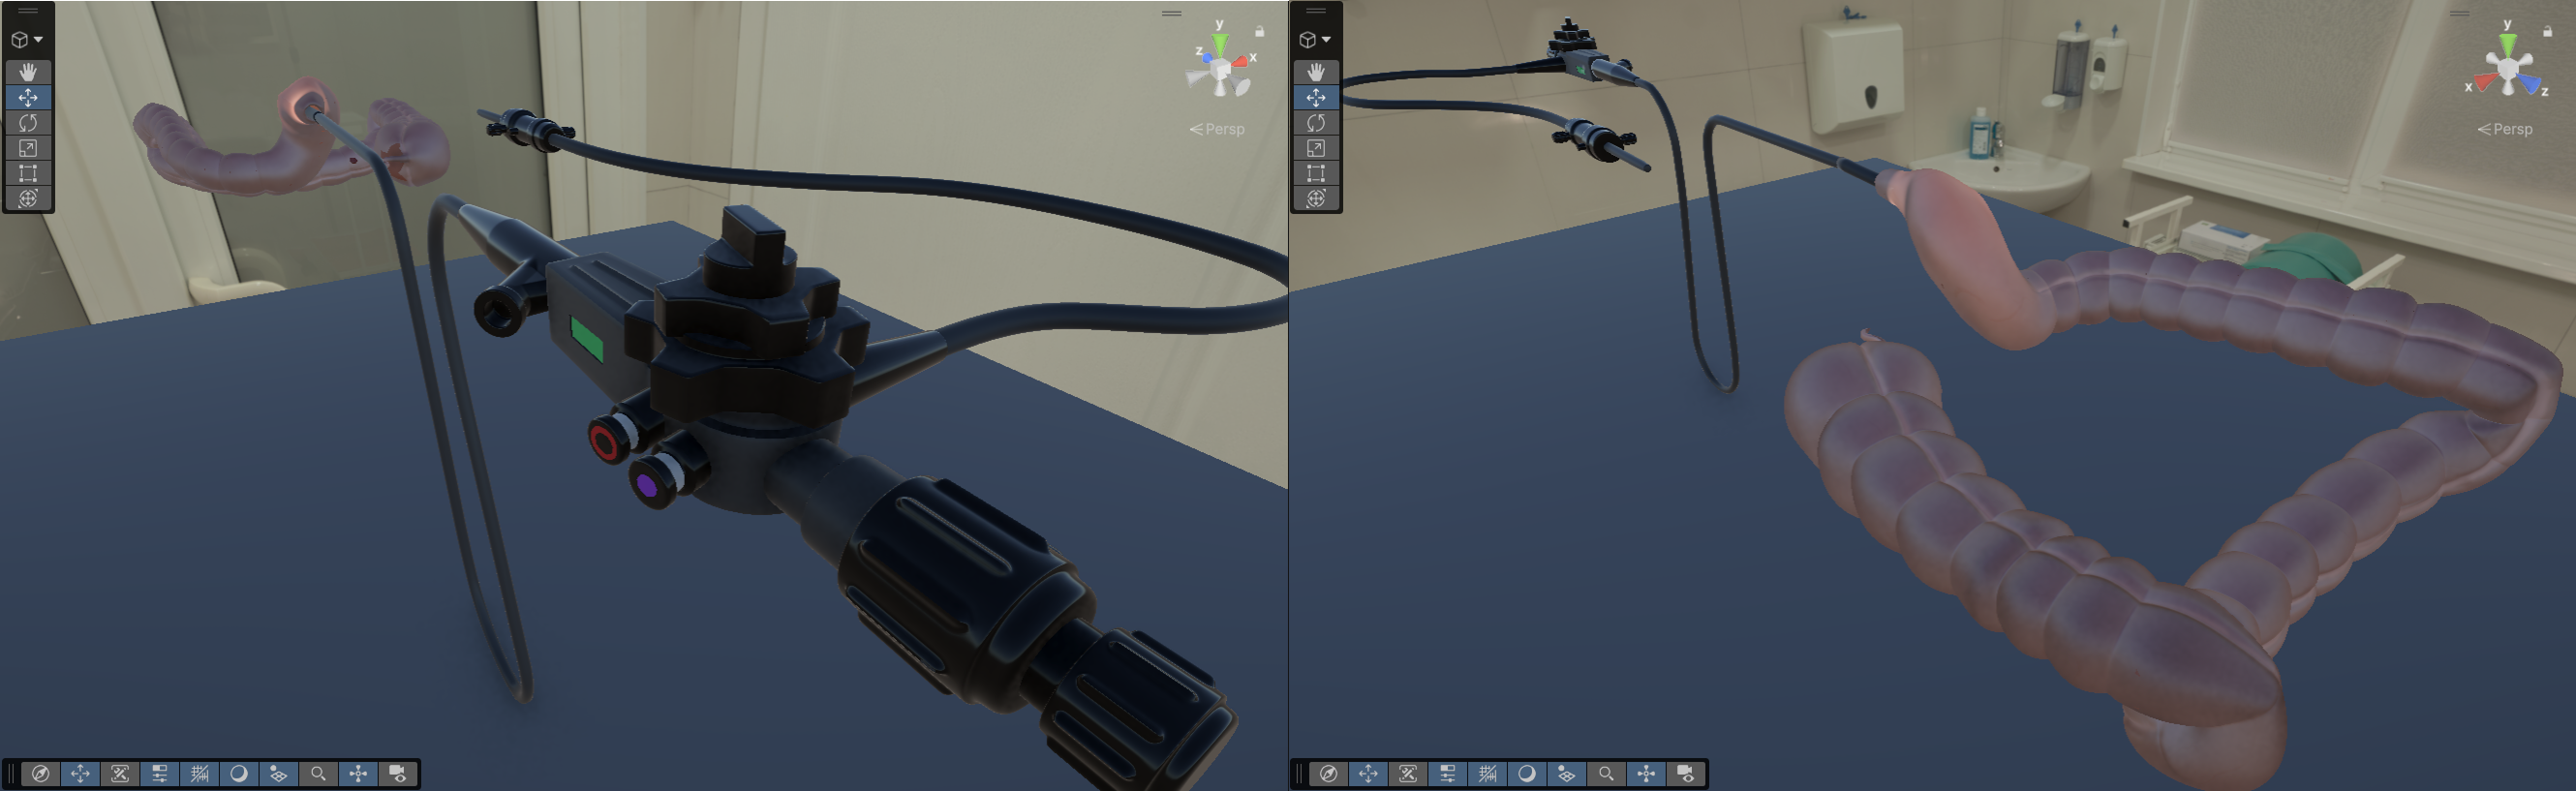
\includegraphics[width=0.8\linewidth]{assets/model-phase1-setup.png}
\caption{The Phase 1 environment: The setup for both the endoscope, its head, and the colon.}
\label{fig:phase1_setup}
\end{figure}

\subsection{The Procedural Forward Push}
Instead of making the agent learn when and how hard to push forward, we wanted to perfectly mimic how a real doctor operates. A human endoscopist doesn't just jam the scope forward at constant speed. They push in short, controlled bursts, pause to look around, and then push again.

To recreate this, we wrote a script called \texttt{EndoscopeBurstPusher}. It uses a procedural, \textbf{jitter-based burst algorithm}:

\begin{equation}
T_{push} = 1.0 + \text{Uniform}(-\delta_{push}, \delta_{push})
\end{equation}
\begin{equation}
T_{pause} = 4.0 + \text{Uniform}(-\delta_{pause}, \delta_{pause})
\end{equation}

The pusher drives the camera forward for a base duration of \textbf{1.0 second at 80\% strength}, then pauses for \textbf{4.0 seconds}. By adding random jitter ($\delta$), we guarantee the agent never memorizes a specific rhythm. It has to constantly read the visual feed to know when it is moving and when it is stationary. The push applies a steady, clinically safe \textbf{2\,cm/s} forward velocity along the pre-calculated centerline spline.

\subsection{The Action Space \& Kinematics}
While the script pushes, the agent's only job is to steer the camera tip to avoid crashing into the pink mucosal walls. We gave the agent a \textbf{single discrete branch} with exactly \textbf{5 actions}. The steering commands are mapped through a script called \texttt{EndoscopeActionDriver}, which translates the discrete choice into a 2D steer input applying rotational torques to the articulated tip joint.

\begin{table}[H]
\centering
\caption{Phase 1: Discrete Action Space Mapping}
\label{tab:p1_actions}
\begin{tabular}{|c|l|l|}
\rowcolor{primary}
\textcolor{white}{\textbf{Discrete Value}} & \textcolor{white}{\textbf{Action}} & \textcolor{white}{\textbf{Resulting Torque Vector}} \\
\hline
0 & Do Nothing & $(0, 0)$ \\
\hline
1 & Pitch Up (W) & $(1, 0)$ \\
\hline
2 & Yaw Left (A) & $(0, -1)$ \\
\hline
3 & Pitch Down (S) & $(-1, 0)$ \\
\hline
4 & Yaw Right (D) & $(0, 1)$ \\
\hline
\end{tabular}
\end{table}


\begin{figure}[H]
\centering
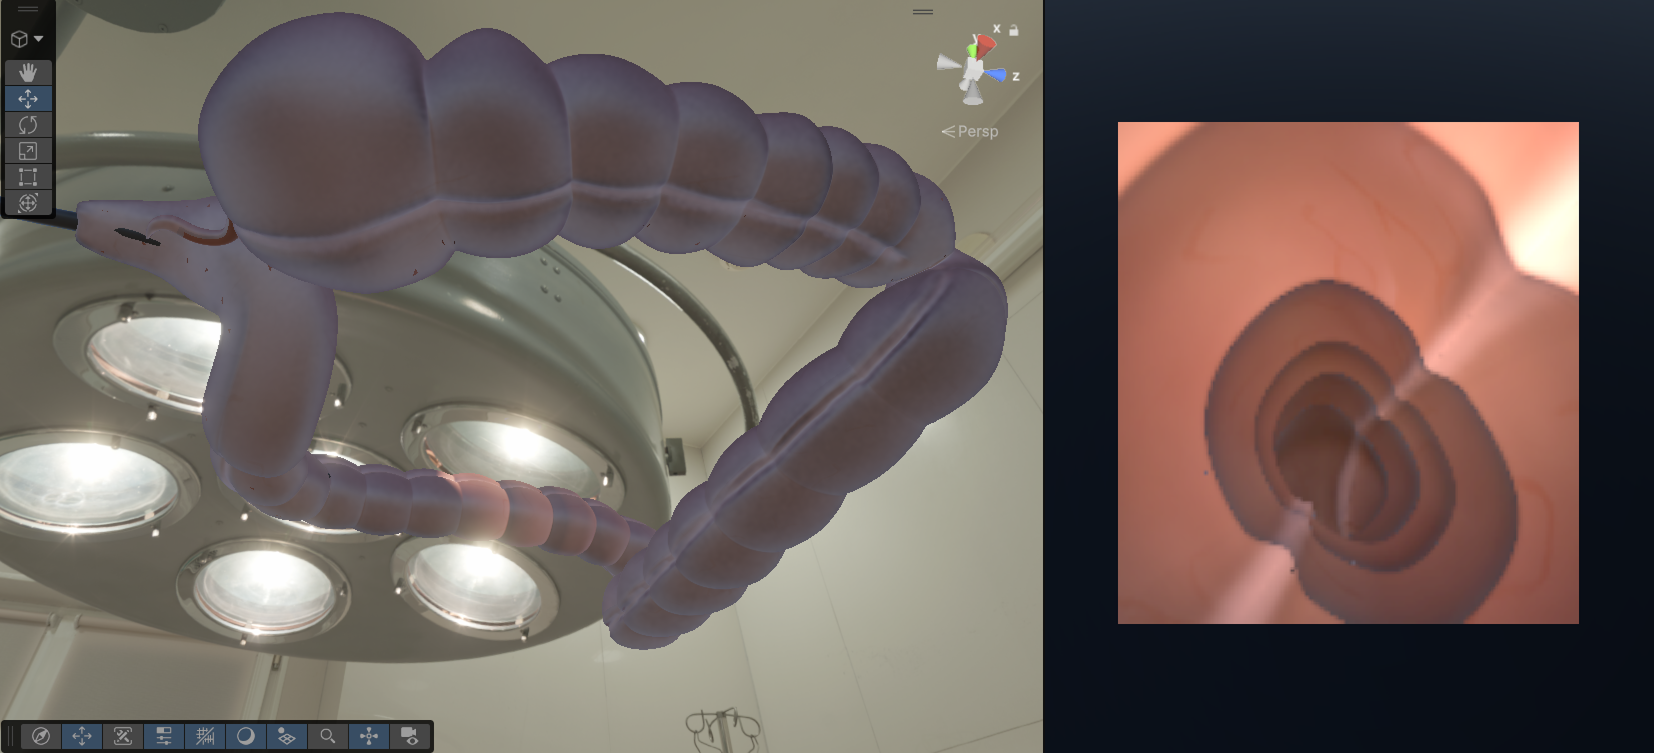
\includegraphics[width=0.8\linewidth]{assets/model-phase1-agent-running.png}
\caption{Phase 1 agent mid-navigation: external colon view (left) and the agent's $128 \times 128$ camera observation (right), showing haustral folds, specular highlights, and the dark distal lumen.}
\label{fig:phase1_running}
\end{figure}

\subsection{State Space \& The CNN/LSTM Brain}
The agent is completely \textbf{vision-only}. No coordinates, no radar, no cheat codes. It sees through a tiny RGB camera feed and has to figure out depth and curves purely from the visual \textbf{optic flow} scrolling past the lens. 

To ensure perfect consistency between training in Python and inference in the virtual simulation, we strictly locked the runtime settings in code: \texttt{Time.captureFramerate = 60}, \textbf{quality level 1}, and forced the screen resolution to exactly $128 \times 128$.

The brain architecture is a pipeline of three stages:
\begin{enumerate}
\item \textbf{CNN Visual Encoder (SimpleVisualEncoder):} Three convolutional layers crunch the $128 \times 128$ RGB image into a compact \textbf{256-dimensional feature vector}. The first Conv2D layer uses \textbf{16 filters} with an $8 \times 8$ kernel and stride 4 (using \textbf{LeakyReLU} activation). The second uses \textbf{32 filters} with a $4 \times 4$ kernel and stride 2. After flattening ($8 \times 8 \times 32 = 2048$ values), a dense layer compresses everything down to 256 features.
\item \textbf{Body MLP (LinearEncoder):} Two fully connected layers of \textbf{256 units each} with \textbf{Swish} activation refine the features.
\item \textbf{LSTM Memory:} A single-layer LSTM with \textbf{sequence length 64} and \textbf{memory size 128} (hidden size 64). This is the secret sauce! The colon is a highly aliased environment - one pink fleshy tunnel looks identical to another. Without temporal memory, the agent cannot tell if it is moving forward, sliding backward, or stuck in a corner.
\end{enumerate}

The LSTM output feeds into a \textbf{policy head} (a single categorical branch of 5 actions, initialized with Kaiming He Normal at gain 0.1) and a \textbf{value head} (one linear layer for the extrinsic reward stream).

\begin{table}[H]
\centering
\caption{Phase 1: Neural Network Architecture}
\label{tab:p1_network}
\begin{tabular}{|l|l|}
\rowcolor{primary}
\textcolor{white}{\textbf{Component}} & \textcolor{white}{\textbf{Specification}} \\
\hline
Input Resolution & $128 \times 128$ RGB (Vision-only) \\
\hline
Conv Layer 1 & 16 filters, $8 \times 8$ kernel, stride 4, LeakyReLU \\
\hline
Conv Layer 2 & 32 filters, $4 \times 4$ kernel, stride 2, LeakyReLU \\
\hline
Flatten $\rightarrow$ Dense & $2048 \rightarrow 256$, LeakyReLU \\
\hline
Body MLP & 2 layers $\times$ 256 units, Swish activation \\
\hline
LSTM Memory & Sequence Length: 64, Memory Size: 128 \\
\hline
Policy Head & MultiCategorical [5], Kaiming init (gain 0.1) \\
\hline
Value Head & 1 linear head (extrinsic) \\
\hline
\end{tabular}
\end{table}

\subsection{Reward Shaping \& Mathematical Formulation}
Training this agent was all about getting the \textbf{reward shaping} exactly right. If the rewards are poorly tuned, the agent will find creative ways to exploit the system. We formulated the total reward at timestep $t$ as:

\begin{equation}
R_t = R_{alive} + R_{goal} - P_{collision} - P_{timeout}
\end{equation}

Here is the exact breakdown:
\begin{itemize}
    \item $R_{alive} = +0.001$: A tiny positive reward for every step it survives without crashing. This gently encourages continued exploration.
    \item $R_{goal} = +10.0$: The jackpot! Awarded instantly when the agent successfully reaches the \texttt{GoalTriggerLogger} target deep inside the colon segment.
    \item $P_{collision} = -1.0$: A harsh penalty if it steers into the mucosal wall. The episode terminates instantly via the \texttt{push\_blocked\_latched} flag.
    \item $P_{timeout} = -0.2$: A small penalty if it takes too long and times out before reaching the goal.
\end{itemize}

We added a critical gate called \texttt{rewardAliveOnlyWhenSafe}. Without this, the agent could literally press its face safely against a non-fatal wall and farm those $+0.001$ alive points forever! The script actively checks \texttt{IsTouchingBlockingLayers()} and denies the alive reward if the camera is scraping tissue. Collision detection itself uses \textbf{capsule overlaps} along the endoscope bone chain and a \textbf{sphere-cast clamp} at the tip during push operations.

\subsection{Clever Engineering: Safe Resets \& Fallbacks}
One really annoying problem we ran into was the agent randomly spawning inside the colon mesh when the episode resets. Because the environment is a tight tube, spawning even a millimeter inside the wall causes instant, explosive physics collisions!

To fix this, we wrote a \textbf{30-step backoff algorithm} called \texttt{ResolveSafeResetPose()}. When the episode begins, if the agent detects it spawned inside a wall, it incrementally backs off by 0.01 units along the opposite direction of its forward vector, checking for collisions at each step. It repeats this up to 30 times until it finds a safe, empty spot to start.

We also added a safety net called \texttt{autoRequestDecisionsIfMissing}. If the \texttt{DecisionRequester} component breaks or gets deleted in the editor, our agent will manually poll for decisions every 5 physics ticks using an internal \texttt{\_fallbackDecisionCounter}, ensuring it never stops driving.


\begin{figure}[H]
\centering
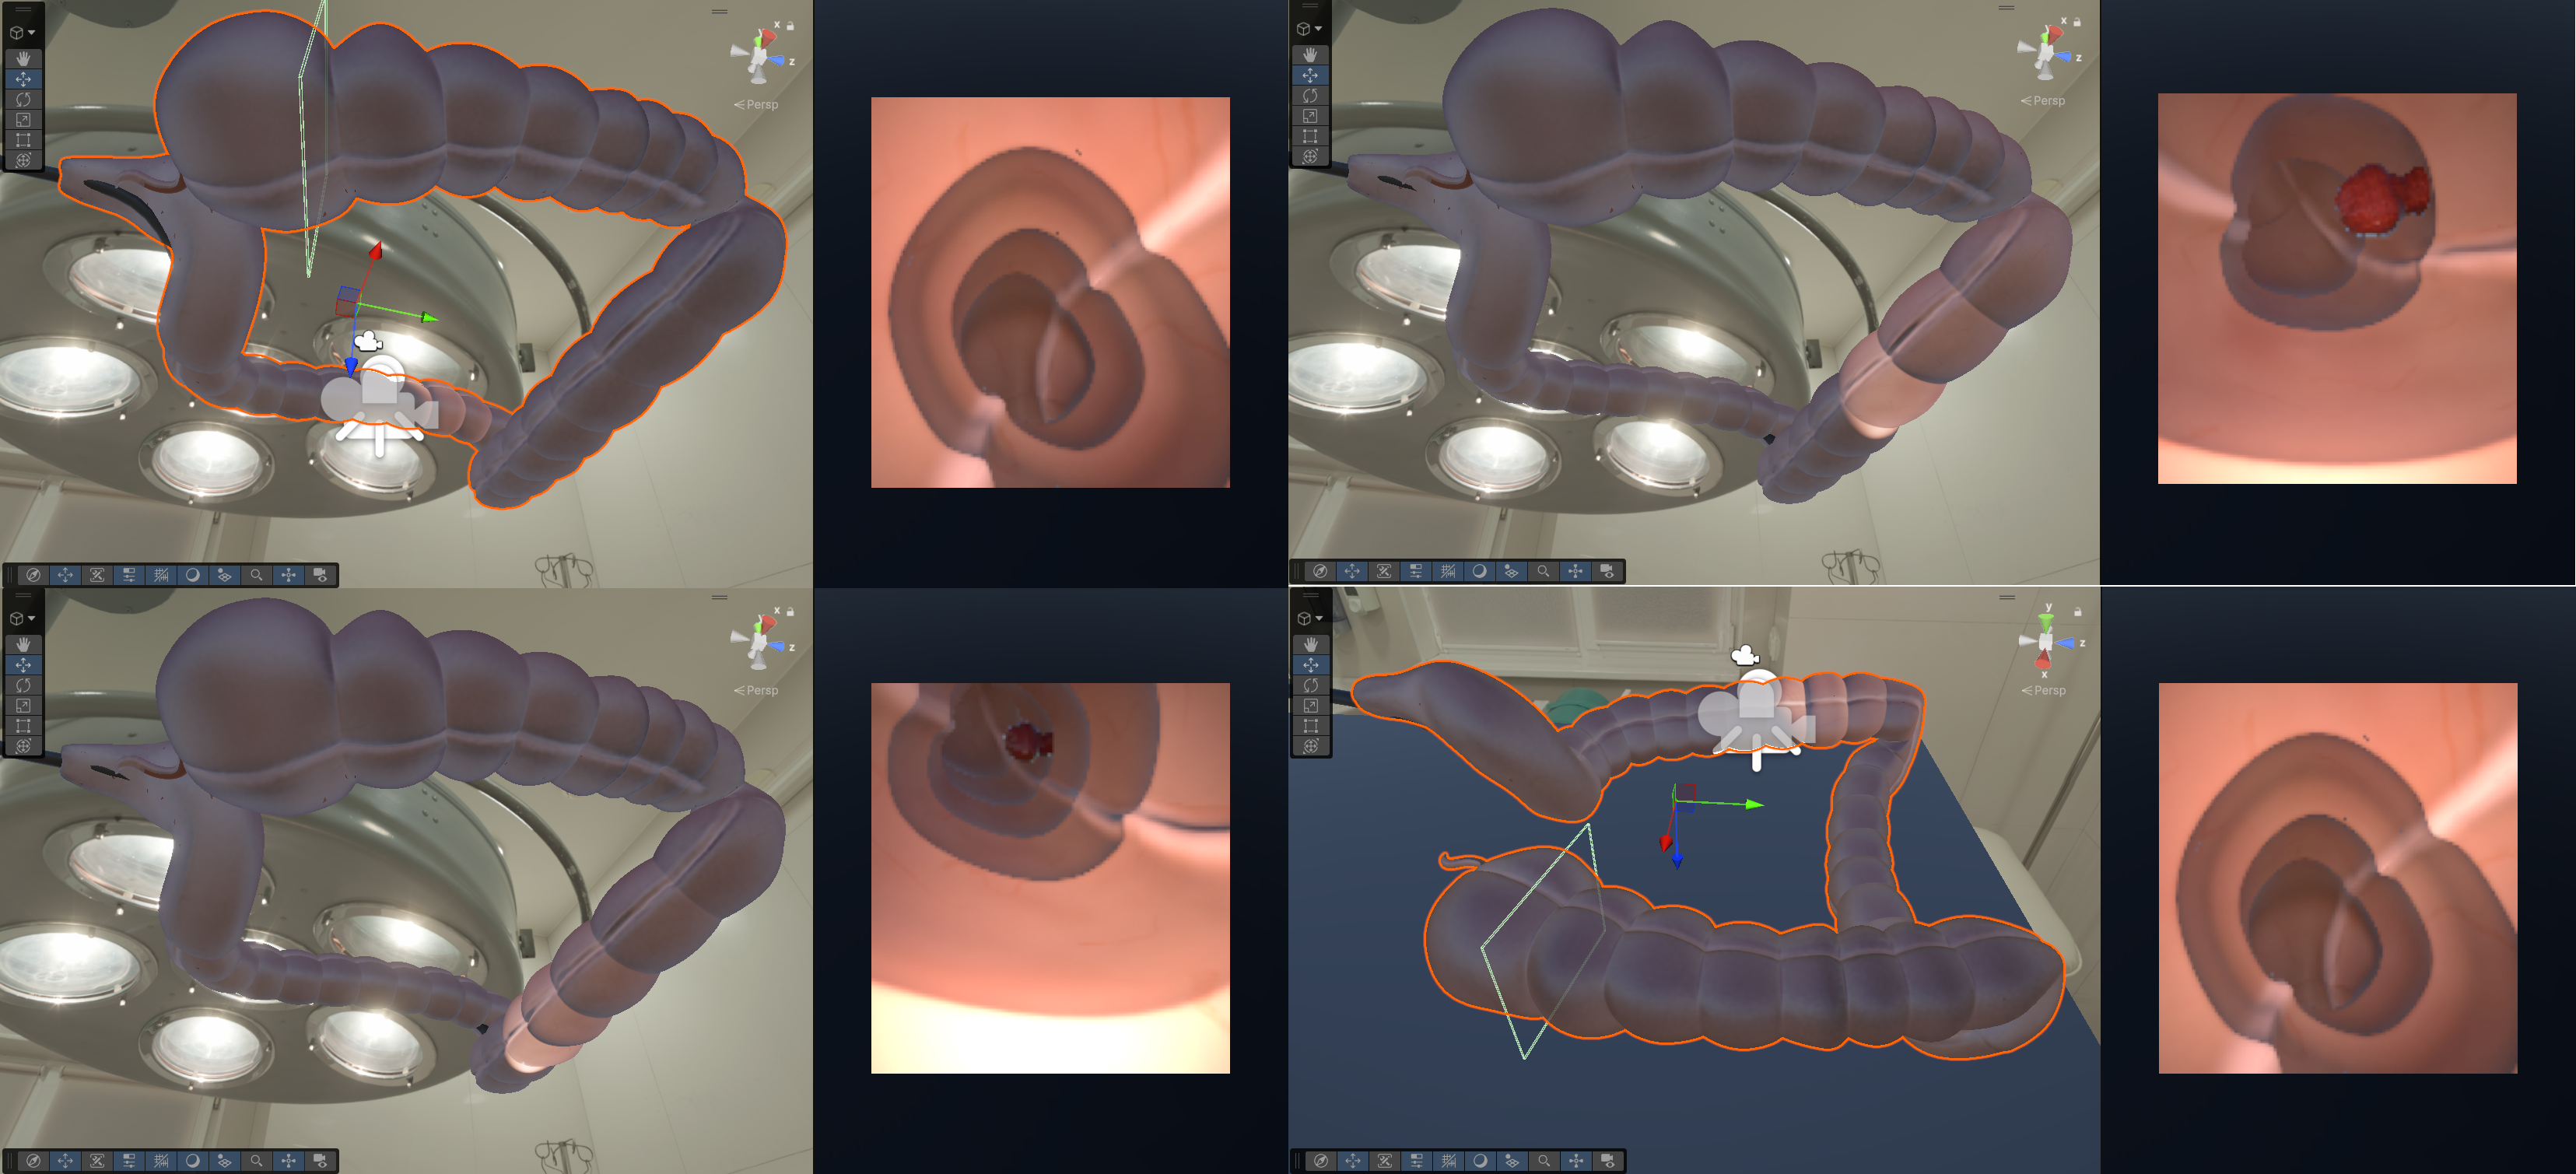
\includegraphics[width=0.8\linewidth]{assets/model-phase1-different-angels.png}
\caption{Multiple perspectives during Phase 1 training. Each panel shows the external environment view alongside the agent's $128 \times 128$ camera feed, demonstrating the diverse visual scenarios the CNN must learn to handle.}
\label{fig:phase1_angles}
\end{figure}

\subsection{Training Hyperparameters}
For training, we used \textbf{Proximal Policy Optimization (PPO)} with a \textbf{linear learning rate schedule}. Because the navigation phase requires seeing a vast amount of visual data to understand the complex curves, we used a large batch size and trained for a total of \textbf{20 million steps}.

\begin{table}[H]
\centering
\caption{Phase 1: PPO Training Hyperparameters}
\label{tab:p1_hyperparameters}
\begin{tabular}{|l|l|}
\rowcolor{primary}
\textcolor{white}{\textbf{Hyperparameter}} & \textcolor{white}{\textbf{Value}} \\
\hline
Algorithm & PPO (Proximal Policy Optimization) \\
\hline
Batch Size & 1024 \\
\hline
Buffer Size & 10,240 \\
\hline
Learning Rate & $3 \times 10^{-4}$ (linear schedule) \\
\hline
Entropy Bonus ($\beta$) & $1 \times 10^{-3}$ \\
\hline
Clip Range ($\epsilon$) & 0.2 \\
\hline
GAE $\lambda$ & 0.95 \\
\hline
Epochs per Update & 3 \\
\hline
Time Horizon & 128 \\
\hline
Max Training Steps & 20,000,000 \\
\hline
Discount ($\gamma$) & 0.99 \\
\hline
Reward Signal & Extrinsic only (strength 1.0) \\
\hline
\end{tabular}
\end{table}

By tuning these parameters carefully, the agent learned to smoothly navigate complex colon geometry without relying on any external positioning sensors - paving the way perfectly for Phase 2!

\subsection{The ``20-Agent Crash''}
Training an RL agent is never a straightforward path. Initially, we tried to drastically speed up the process by spawning \textbf{20 agents simultaneously} and running the simulation at $20\times$ speed. Unfortunately, Unity struggled to distribute the physics load, bottlenecking on a single CPU core. This caused major instability and forced us to rewrite significant chunks of the environment. When twenty endoscopes interacted with twenty colon meshes simultaneously at hyperspeed, the physics engine collapsed. Frame drops allowed the endoscopes to physically tunnel through the colon walls into the virtual void. Worse, because RL strictly synchronizes physics with action steps, these lag spikes corrupted the neural network's observation buffer. The agent began receiving observations that were completely desynchronized from its actions, forcing it to learn from a chaotic, delayed reality. This bottleneck revealed a crucial lesson: brute-forcing parallel environments is counterproductive if the underlying physics engine cannot guarantee strict, deterministic execution. Consequently, we had to completely abandon our ambitious multi-agent setup.

\subsection{Training Results}
Eventually, we pivoted to a \textbf{single-agent training pipeline}. This let us carefully observe the agent's behavior during each run and iteratively tweak \textbf{hyperparameters} and \textbf{reward structures}. It took \textbf{15 complete retrain attempts} - with each run lasting anywhere from 8 to 30 hours - before we finally discovered the \textbf{golden configuration} that produced a reliable, \textbf{collision-free driving policy}. For Phase 1, the agent ultimately achieved a \textbf{best score of 14.67}, taking \textbf{6.5 million steps} over a grueling \textbf{4 days} of training. By isolating the training to a single environment, we avoided the catastrophic forgetting and unstable gradients that plagued our earlier multi-agent asynchronous approaches. The resulting policy demonstrated remarkable robustness, smoothly navigating the tightest haustral flexures without triggering the collision penalties. Figure~\ref{fig:nav_dashboard} displays the telemetry and learning curves from this definitive run.

\begin{figure}[H]
\centering
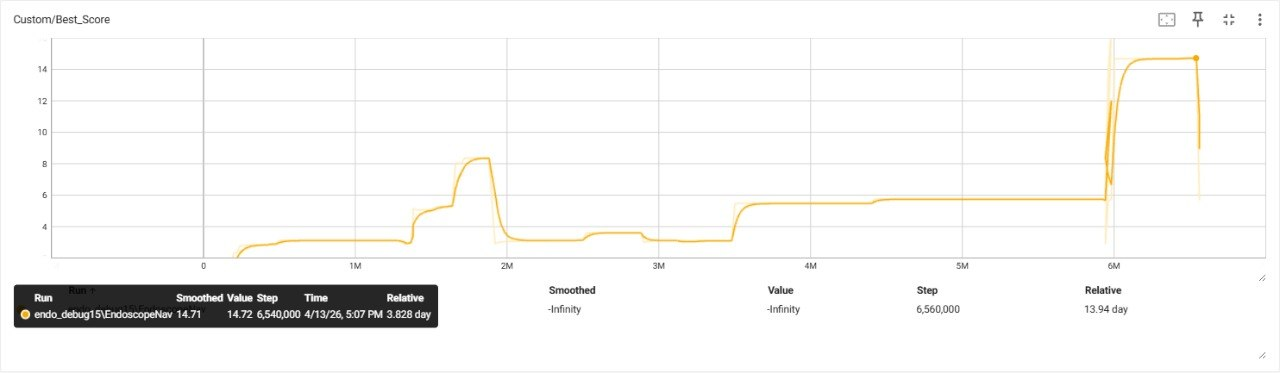
\includegraphics[width=1\linewidth]{assets/dashboard-3.jpg}
\caption{Training telemetry dashboard for Phase 1, showing the convergence of cumulative reward and episode length over 6.5 million steps.}
\label{fig:nav_dashboard}
\end{figure}

\clearpage
